\begin{frame}
  \frametitle{MD5}
  \begin{minipage}[t]{0.45\linewidth}
    Points about MD5:
    \begin{itemize}
    \item Point one
    \item Point two
    \item Point three
    \end{itemize}
  \end{minipage}\hfill
  \begin{minipage}[t][3cm][c]{0.5\linewidth}
    \centering
    \begin{figure}
      \centering
      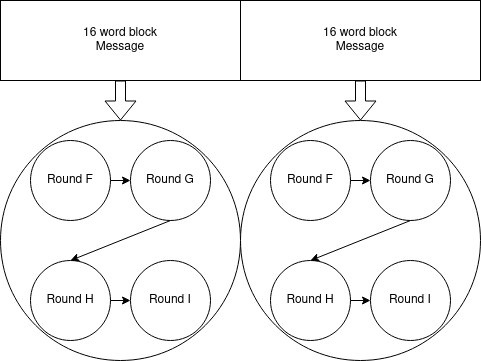
\includegraphics[width=\textwidth]{RoundsMD5}
      \caption{MD5 round}
    \end{figure}
  \end{minipage}

  \begin{minipage}[b][4cm][b]{0.9\linewidth}
  \begin{figure}
    \centering
    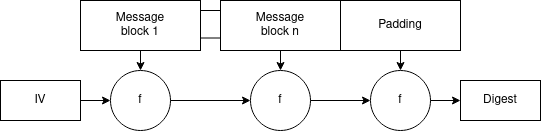
\includegraphics[width=0.95\textwidth]{merkle1}
    \caption{Merkle-Damgaard construction}
  \end{figure}
  \end{minipage}

\end{frame}

% \begin{frame}
% \frametitle{MD5}
% \end{frame}